\documentclass{article}
\usepackage{physics}
\usepackage{graphicx}
\usepackage{caption}
\usepackage{amsmath}
\usepackage{bm}
\usepackage{framed}
\usepackage{authblk}
\usepackage{empheq}
\usepackage{amsfonts}
\usepackage{esint}
\usepackage[makeroom]{cancel}
\usepackage{dsfont}
\usepackage{centernot}
\usepackage{mathtools}
\usepackage{subcaption}
\usepackage{bigints}
\usepackage{amsthm}
\theoremstyle{definition}
\newtheorem{lemma}{Lemma}
\newtheorem{defn}{Definition}[section]
\newtheorem{prop}{Proposition}[section]
\newtheorem{rmk}{Remark}[section]
\newtheorem{thm}{Theorem}[section]
\newtheorem{exmp}{Example}[section]
\newtheorem{prob}{Problem}[section]
\newtheorem{sln}{Solution}[section]
\newtheorem*{prob*}{Problem}
\newtheorem{exer}{Exercise}[section]
\newtheorem*{exer*}{Exercise}
\newtheorem*{sln*}{Solution}
\usepackage{empheq}
\usepackage{tensor}
\usepackage{xcolor}
%\definecolor{colby}{rgb}{0.0, 0.0, 0.5}
\definecolor{MIT}{RGB}{163, 31, 52}
\usepackage[pdftex]{hyperref}
%\hypersetup{colorlinks,urlcolor=colby}
\hypersetup{colorlinks,linkcolor={MIT},citecolor={MIT},urlcolor={MIT}}  
\usepackage[left=1in,right=1in,top=1in,bottom=1in]{geometry}
\setcounter{MaxMatrixCols}{20}
\usepackage{newpxtext,newpxmath}
\newcommand*\widefbox[1]{\fbox{\hspace{2em}#1\hspace{2em}}}

\newcommand{\p}{\partial}
\newcommand{\R}{\mathbb{R}}
\newcommand{\C}{\mathbb{C}}
\newcommand{\lag}{\mathcal{L}}
\newcommand{\nn}{\nonumber}
\newcommand{\ham}{\mathcal{H}}
\newcommand{\M}{\mathcal{M}}
\newcommand{\I}{\mathcal{I}}
\newcommand{\K}{\mathcal{K}}
\newcommand{\F}{\mathcal{F}}
\newcommand{\w}{\omega}
\newcommand{\lam}{\lambda}
\newcommand{\al}{\alpha}
\newcommand{\be}{\beta}
\newcommand{\x}{\xi}

\newcommand{\G}{\mathcal{G}}

\newcommand{\f}[2]{\frac{#1}{#2}}

\newcommand{\ift}{\infty}

\newcommand{\lp}{\left(}
\newcommand{\rp}{\right)}

\newcommand{\lb}{\left[}
\newcommand{\rb}{\right]}

\newcommand{\lc}{\left\{}
\newcommand{\rc}{\right\}}


\newcommand{\V}{\mathbf{V}}
\newcommand{\U}{\mathcal{U}}
\newcommand{\Id}{\mathcal{I}}
\newcommand{\D}{\mathcal{D}}
\newcommand{\Z}{\mathcal{Z}}

%\setcounter{chapter}{-1}


\usepackage{enumitem}



\usepackage{listings}
\captionsetup[lstlisting]{margin=0cm,format=hang,font=small,format=plain,labelfont={bf,up},textfont={it}}
\renewcommand*{\lstlistingname}{Code \textcolor{violet}{\textsl{Mathematica}}}
\definecolor{gris245}{RGB}{245,245,245}
\definecolor{olive}{RGB}{50,140,50}
\definecolor{brun}{RGB}{175,100,80}

%\hypersetup{colorlinks,urlcolor=colby}
\lstset{
	tabsize=4,
	frame=single,
	language=mathematica,
	basicstyle=\scriptsize\ttfamily,
	keywordstyle=\color{black},
	backgroundcolor=\color{gris245},
	commentstyle=\color{gray},
	showstringspaces=false,
	emph={
		r1,
		r2,
		epsilon,epsilon_,
		Newton,Newton_
	},emphstyle={\color{olive}},
	emph={[2]
		L,
		CouleurCourbe,
		PotentielEffectif,
		IdCourbe,
		Courbe
	},emphstyle={[2]\color{blue}},
	emph={[3]r,r_,n,n_},emphstyle={[3]\color{magenta}}
}

\newcommand{\diag}{\text{diag}}
\newcommand{\psirot}{\ket{\psi_\text{rot}(t)} }
\newcommand{\RWA}{\ham_\text{rot}^\text{RWA}}


\begin{document}
\begin{framed}
\noindent Name: \textbf{Huan Q. Bui}\\
Course: \textbf{8.421 - AMO I}\\
Problem set: \textbf{\#5}\\
Due: Friday, March 11, 2022.
\end{framed}



\noindent \textbf{1. Magnetic field of a magnetic dipole}


\begin{enumerate}[label=(\alph*)]
	\item From the identity
	\begin{align*}
	\p_i \p_j \lp \f{1}{r} \rp = -\p_i \lp \f{\hat{\bm{r}}_j}{r^2} \rp = -\p_i \lp \f{x_j}{r^3} \rp = \f{3 \hat{\bm{r}}_i \hat{\bm{r}}_j - \delta_{ij}}{r^3} - \f{4\pi}{3} \delta_{ij} \delta^3(\bm{r}),
	\end{align*}
	we simply contract to get
	\begin{align*}
	\nabla^2 \lp \f{1}{r} \rp 
	&= \sum_{i=1}^3 \p_i \p_i \lp \f{1}{r} \rp \\
	&=  \sum_{i=1}^3 \f{3 \hat{\bm{r}}_i \hat{\bm{r}}_i - \delta_{ii}}{r^3} - \f{4\pi}{3} \delta_{ii} \delta^3(\bm{r}) \\
	&= \sum_{i=1}^3 \f{3 \hat{\bm{r}}_i \hat{\bm{r}}_i - 1}{r^3} - \f{4\pi}{3} \delta^3(\bm{r}) \\
	&= \f{3(x^2+y^2+z^2)/r^2-3}{r^3} - 4\pi \delta^3(\bm{r})\\
	&= \f{3r^2/r^2-3}{r^3} - 4\pi \delta^3(\bm{r})\\
	&= -4\pi \delta^3(\bm{r})
	\end{align*}
	as desired. Note that here $\delta_{ii}=1$ is a matrix element since we are not using Einstein summation convention here. We will use it in the next part of the problem, however.  
	
	
	\item Let the vector potential for a magnetic dipole be given 
	\begin{align*}
	\bm{A}^\text{dip}(\bm{r}) = \f{\bm{m} \times \hat{\bm{r}}}{r^2}.
	\end{align*}
	For ease of computation, we may rewrite this using the Levi-Civita symbol and Einstein summation convention:
	\begin{align*}
	\bm{A}^\text{dip}_i(\bm{r}) = \f{1}{r^2}\epsilon_{ijk} \bm{m}_j \hat{\bm{r}}_k 
	\end{align*}
	The magnetic field of a magnetic dipole is thus given by taking the curl of $\bm{A}_\text{dip}$, by definition:
	\begin{align*}
	\bm{B}^\text{dip}_a(\bm{r}) 
	&= [\bm{\nabla}\times \bm{A}^\text{dip}(\bm{r})]_a \\
	&= \epsilon_{abc} \p_b \bm{A}^\text{dip}_c(\bm{r})\\
	&= \epsilon_{abc} \p_b \lp \f{1}{r^2}\epsilon_{cjk} \bm{m}_j \hat{\bm{r}}_k  \rp\\
	&= \epsilon_{abc}\epsilon_{cjk} \bm{m}_j \p_b \lp \f{\hat{\bm{r}}_k}{r^2}  \rp.
	\end{align*}
	Using the identity given in the problem statement and the fact that
	\begin{align*}
	\epsilon_{abc}\epsilon_{cjk} = \epsilon_{cab}\epsilon_{cjk} = \delta_{aj}\delta_{bk} - \delta_{ak}\delta_{bj}
	\end{align*}
	we have
	\begin{align*}
	\bm{B}^\text{dip}_a(\bm{r}) &= -(\delta_{aj}\delta_{bk} - \delta_{ak}\delta_{bj})\, \bm{m}_j \p_b \p_k  \lp \f{1}{r}  \rp\\
	&= -(\delta_{aj}\delta_{bk} - \delta_{ak}\delta_{bj})\, \bm{m}_j \lp \f{3 \hat{\bm{r}}_b \hat{\bm{r}}_k - \delta_{bk}}{r^3} - \f{4\pi}{3} \delta_{bk} \delta^3(\bm{r})  \rp\\
	&= -\delta_{aj}\delta_{bk} \bm{m}_j \lp \f{3 \hat{\bm{r}}_b \hat{\bm{r}}_k - \delta_{bk}}{r^3} - \f{4\pi}{3} \delta_{bk} \delta^3(\bm{r})  \rp + \delta_{ak}\delta_{bj}\bm{m}_j \lp \f{3 \hat{\bm{r}}_b \hat{\bm{r}}_k - \delta_{bk}}{r^3} - \f{4\pi}{3} \delta_{bk} \delta^3(\bm{r})  \rp\\
	&= -\bm{m}_a \lp \cancel{\f{3 \hat{\bm{r}}_b \hat{\bm{r}}_b - \delta_{bb}}{r^3}} - \f{4\pi}{3} \delta_{bb} \delta^3(\bm{r})  \rp + \bm{m}_b \lp \f{3 \hat{\bm{r}}_b \hat{\bm{r}}_a - \delta_{ba}}{r^3} - \f{4\pi}{3} \delta_{ba} \delta^3(\bm{r})  \rp \\
	&= \bm{m}_a 4\pi \delta^3(\bm{r})    +   \f{3 (\bm{m}_b\hat{\bm{r}}_b) \hat{\bm{r}}_a - \bm{m}_a}{r^3} - \f{4\pi}{3} \bm{m}_a \delta^3(\bm{r})   \\
	&=   \f{3 (\bm{m}\cdot \hat{\bm{r}}) \hat{\bm{r}}_a - \bm{m}_a}{r^3} + \f{8\pi}{3} \bm{m}_a \delta^3(\bm{r}),
	\end{align*}
	where we have used the contraction identity $\delta_{ii}=3$.  Putting back into vector form, we find 
	\begin{align*}
	\bm{B}^\text{dip}(\bm{r}) =  \f{3 (\bm{m}\cdot \hat{\bm{r}}) \hat{\bm{r}} - \bm{m}}{r^3} + \f{8\pi}{3} \bm{m} \delta^3(\bm{r})
	\end{align*}
	as desired. 
	
	
	
	\item It remains to prove the provided identity:
	\begin{align*}
	\p_i \p_j \lp \f{1}{r} \rp = -\p_i \lp \f{\hat{\bm{r}}_j}{r^2} \rp = -\p_i \lp \f{x_j}{r^3} \rp = \f{3 \hat{\bm{r}}_i \hat{\bm{r}}_j - \delta_{ij}}{r^3} - \f{4\pi}{3} \delta_{ij} \delta^3(\bm{r}),
	\end{align*}
	
	The first two equalities are straightforward to show, but I will show the proofs here anyway as the technique carries over to proving the third equality (which is the one we really care about):
	\begin{align*}
	\p_i \p_j \lp \f{1}{r} \rp 
	&= \p_i \p_j \f{1}{\lp \sum_{a=1}^3 x_a^2 \rp^{1/2}} \\
	&= -\p_i\lb \f{1}{2\lp \sum_{a=1}^3 x_a^2 \rp^{3/2}} \p_j \lp \sum_{a=1}^3  x_a\rp\rb\\
	&= -\p_i\lb \f{1}{2r^3} \sum_{a=1}^3 2x_a \delta_{ja}\rb\\
	&= -\p_i\lp \f{x_j}{r^3} \rp\\
	&= -\p_i\lp \f{\hat{\bm{r}}_j}{r^2} \rp.
	\end{align*}
	where we have used $x_j = r \hat{\bm{r}}_j$. Now we focus on the last equality. We will consider two cases. For $r\neq 0$, we may prove the identity above but ignoring the $\delta$-function piece: 
	\begin{align*}
	\p_i \p_j \lp \f{1}{r} \rp = -\p_i \lp \f{\hat{\bm{r}}_j}{r^2} \rp = -\p_i \lp \f{x_j}{r^3} \rp = \f{3 \hat{\bm{r}}_i \hat{\bm{r}}_j - \delta_{ij}}{r^3}.
	\end{align*}
	To prove this, we simply calculate away:
	\begin{align*}
	\p_i \p_j \lp \f{1}{r} \rp &= -\p_i \lp \f{\hat{\bm{r}}_j}{r^2} \rp \\
	&= -\p_i \lp \f{x_j}{r^3} \rp \\
	&= \f{-\p_i x_j}{r^3} - x_j \p_i \f{1}{r^3}\\
	&= -\f{\delta_{ij}}{r^3} - x_j \p_i \f{1}{\lp \sum_{a=1}^3 x_a^2 \rp^{3/2}}\\
	&= -\f{\delta_{ij}}{r^3} + \f{3}{2} \f{x_j}{r^5} \p_i \lp \sum_{a=1}^3 x_a^2 \rp\\
	&= -\f{\delta_{ij}}{r^3} + \f{3}{2} \f{x_j}{r^5} \lp \sum_{a=1}^3 2 x_a \delta_{ia} \rp\\
	&= -\f{\delta_{ij}}{r^3} + \f{3 x_i x_j}{r^5}\\
	&= \f{3 \hat{\bm{r}}_i \hat{\bm{r}}_j - \delta_{ij}}{r^3}.
	\end{align*}
	And we're done. 
	
	
	Now consider the case where $r$ can be $0$. We will calculate $\p_i \p_j (1/r)$ via integration rather than taking derivatives. To this end, we make use of Gauss-Ostrogradsky theorem for volume integral of a gradient field:
	\begin{align*}
	\int_V \grad \psi \,dV = \int_{\p V} \psi \bm{n} \,da.
	\end{align*}
	In index notation, this is 
	\begin{align*}
	\int_V \p_i \psi \,dV = \int_{\p V} \psi \bm{n}_i \,da.
	\end{align*}
	Let $\psi = \hat{\bm{r}}_j / r^2$ and the volume $V$ to be that of a sphere centered at the origin with radius $\epsilon$. We have that
	\begin{align*}
	I_{ij} &= \int_V  \p_i \lp \f{\hat{\bm{r}}_j}{r^2}\rp \,dV \\
	&= \int_{\p V} \f{\hat{\bm{r}}_j \hat{\bm{r}}_i }{r^2} \,da \\
	&= \int_{\p V, r=\epsilon} \f{\hat{\bm{r}}_j  \hat{\bm{r}}_i }{r^2}r^2\sin\theta\,dr d\theta d\phi\\
	&= \int_{\p V, r=\epsilon} \f{x_i x_j}{r^2}\sin\theta\,dr d\theta d\phi.
	\end{align*}
	At this point one may argue that due to spherical symmetry, only the diagonal terms $i=j$ are nonzero and are equal to a third of the trace. It then suffices to find the trace using the usual form of the Gauss-Ostrogradsky theorem. Here, I will present an explicit calculation of the (tensor) elements by expressing $x_i$ in spherical coordinates. 
	\begin{align*}
	&x = \epsilon\sin\theta\cos\phi \\
	&y = \epsilon\sin\theta\cos\phi\\
	&z = \epsilon\cos\theta.
	\end{align*}
	Using Mathematica (this is really not necessary since we can tell which integrand is odd/even... but for completeness I will just show everything explicitly):
	\begin{align*}
	&I_{xx} = I_{yy} = I_{zz} = \f{4\pi}{3} \\
	&I_{xy} = I_{yx} = I_{xz} = I_{zx} = I_{yz} = I_{zy} = 0.
	\end{align*}
	With this, we're done. Putting everything together, we find that
	\begin{align*}
	I_{ij} = \f{4\pi}{3}\delta_{ij}.
	\end{align*}
	Using the same technique\footnote{This integral diverges and therefore requires \textit{regularization} in the sense that integration over the angular variables is carried out first, giving zero, rendering the radial integration unnecessary. The Mathematica code in the box has only integration over $\theta,\phi$.} (or in view of Gauss-Ostrogradsky theorem), we can also show that 
	\begin{align*}
	\int_V \f{3 \hat{\bm{r}}_i \hat{\bm{r}}_j - \delta_{ij}}{r^3}\,dV = 0.
	\end{align*}
	Therefore the condition that 
	\begin{align*}
	-\int_V \p_i \p_j \f{1}{r} = \int_V  \p_i \lp \f{\hat{\bm{r}}_j}{r^2}\rp\,dV = \f{4\pi}{3}\delta_{ij} \quad \text{if } {0 \in V} 
	\end{align*}
	is only satisfied if $\p_i \p_j (1/r)$ has a Dirac $\delta$-function piece in addition to the usual ``dipole'' piece which doesn't contribute to the integral over $V \ni 0$:
	\begin{align*}
	\p_i \p_j \lp \f{1}{r} \rp = -\p_i \lp \f{\hat{\bm{r}}_j}{r^2} \rp = -\p_i \lp \f{x_j}{r^3} \rp = \f{3 \hat{\bm{r}}_i \hat{\bm{r}}_j - \delta_{ij}}{r^3} - \f{4\pi}{3} \delta_{ij} \delta^3(\bm{r}).
	\end{align*}
	We have thus proved the identity. \\
	
	
	
	Mathematica code:
	\begin{lstlisting}
	(*Ixx*)
	Integrate[
	r*Cos[p]*Sin[t]*r*Cos[p]*Sin[t]*r^2/r^4*Sin[t], {t, 0, Pi}, {p, 0, 
	2 Pi}]
	
	Out[19]= (4 \[Pi])/3
	
	(*Iyy*)
	Integrate[
	r*Cos[p]*Sin[t]*r*Cos[p]*Sin[t]*r^2*Sin[t]/r^4, {t, 0, Pi}, {p, 0, 
	2 Pi}]
	
	Out[17]= (4 \[Pi])/3
	
	(*Izz*)
	Integrate[
	r^2 Cos[t]^2*r^2*Sin[t]/r^4, {t, 0, Pi}, {p, 0, 2 Pi}]
	
	Out[23]= (4 \[Pi])/3
	
	(*Ixy*)
	Integrate[
	r*Cos[p]*Sin[t]*r*Sin[p]*Sin[t]*r^2/r^4*Sin[t], {t, 0, Pi}, {p, 0, 
	2 Pi}]
	
	Out[29]= 0
	
	(*Iyz*)
	Integrate[
	r*Cos[t]*r*Sin[p]*Sin[t]*r^2/r^4*Sin[t], {t, 0, Pi}, {p, 0, 2 Pi}]
	
	Out[30]= 0
	
	(*Ixz*)
	Integrate[
	r*Cos[t]*r*Sin[p]*Cos[t]*r^2/r^4*Sin[t], {t, 0, Pi}, {p, 0, 2 Pi}]
	
	Out[31]= 0
	
	
	
	
	
	
	(*Dipole stuff... regularization is needed, i.e. I won't do \
	the integral over r. Suffices to integrate over angles*)
	
	(*xx*)
	Integrate[(3*Cos[p]*Sin[t]*Cos[p]*Sin[t] - 1)/r*Sin[t], {t, 
	0, Pi}, {p, 0, 2 Pi}]
	
	Out[36]= 0
	
	(*yy*)
	Integrate[(3*Sin[p]*Sin[t]*Sin[p]*Sin[t] - 1)/r*Sin[t], {t, 
	0, Pi}, {p, 0, 2 Pi}]
	
	Out[39]= 0
	
	(*zz*)
	Integrate[(3*Cos[t] Cos[t] - 1)/r*Sin[t], {t, 0, Pi}, {p, 0, 
	2 Pi}]
	
	Out[40]= 0
	
	(*xy*)
	Integrate[(3*Cos[p]*Sin[t]*Sin[p]*Sin[t])/r*Sin[t], {t, 0, 
	Pi}, {p, 0, 2 Pi}]
	
	Out[44]= 0
	
	(*yz*)
	Integrate[(3*Cos[t]*Sin[t]*Sin[p])/r*Sin[t], {t, 0, Pi}, {p, 
	0, 2 Pi}]
	
	Out[45]= 0
	
	(*xz*)
	Integrate[(3*Cos[t]*Cos[p]*Sin[t])/r*Sin[t], {t, 0, Pi}, {p, 
	0, 2 Pi}]
	
	Out[47]= 0
	
	\end{lstlisting}
	
	
	
\end{enumerate}



\noindent \textbf{2. Atoms in magnetic fields: the Breit-Rabi formula}

$\,$


\noindent The Hamiltonian is 
\begin{align*}
\ham = ah \bm{I}\cdot \bm{J} + (g_J \mu_B m_J - g_I \mu_B m_I) B_z.
\end{align*}



\begin{enumerate}[label=(\alph*)]
	\item We assume that $J=1/2$. To find the eigenenergies for this Hamiltonian for all fields, we have to diagonalize it in some basis. As suggested by the form of the Breit-Rabi formula, let us diagonalize a ``block'' of $\ham$ in which $m = m_F = m_J + m_I$ is fixed (which is possible since $m$ is a good quantum number at any magnetic field). Working in the $\ket{Jm_J Im_I}$ basis, we may write $m_J = \pm 1/2$ which gives $m_I = m_F - m_J = m_F \mp 1/2$. 
	
	Let us compute the matrix elements
	\begin{align*}
	\langle{m_I'm_J'}| \ham |{m_I m_J}\rangle
	\end{align*}  
	for this sub-matrix. This is a $2\times 2$ matrix, so we may as well write down each element explicitly. Before doing anything else, we will recall that
	\begin{align*}
	\bm{I}\cdot \bm{J} = I_xJ_x + I_yJ_y + I_zJ_z = \f{1}{2}(I^+J^- + I^-J^+) + I_z J_z.
	\end{align*}
	Now, let us calculate:
	\begin{align*}
	\,\,&\langle{m_I'm_J'}| \ham |{m_I m_J}\rangle \\
	=\,\,& ah \langle{m_I'm_J'}| \f{1}{2}(I^+J^- + I^-J^+) + I_z J_z |{m_I m_J}\rangle + \langle{m_I'm_J'}|(g_J \mu_B m_J - g_I \mu_B m_I) B_z |{m_I m_J}\rangle \\
	=\,\,& \f{ah}{2}\langle{m_I'm_J'}|  I^+J^- |{m_I m_J}\rangle + \f{ah}{2}\langle{m_I'm_J'}|  I^-J^+ |{m_I m_J}\rangle + (g_J \mu_B m_J - g_I \mu_B m_I) B_z \delta_{m_I'm_I}\delta_{m_J'm_J}\\
	=\,\,& \f{ah}{2}\sqrt{(I-m_I)(I+m_I+1)(J+m_J)(J-m_J+1)}\langle m_I'm_J' | m_I+1,m_J-1\rangle\\
	&\quad +  \f{ah}{2}\sqrt{(I+m_I)(I-m_I+1)(J-m_J)(J+m_J+1)}\langle m_I'm_J' | m_I-1,m_J+1\rangle \\
	&\quad + (g_J \mu_B m_J - g_I \mu_B m_I) B_z \delta_{m_I'm_I}\delta_{m_J'm_J} + ahm_I m_J \delta_{m_I'm_I}\delta_{m_J m_J'}.
	\end{align*}
	With $J=1/2 \implies m_J = \pm 1/2$, we have that the first term is nonzero only for $m_J=1/2 \implies m_I = m_F-1/2 = m-1/2$ and thus $m_J'=-1/2, m_I' = m+1/2$. In this case, it is equal to 
	\begin{align*}
	\f{ah}{2}\sqrt{(I-m+1/2)(I+m-1/2+1)(1/2+1/2)(1/2-1/2+1)} = \f{ah}{2}\sqrt{(I-m+1/2)(I+m+1/2)}.
	\end{align*}
	Similarly, the second term is nonzero only for $m_J = -1/2 \implies m_I = m_F+1/2$ and thus $m_J'=1/2, m_I' = m-1/2$. In this case, it is equal to 
	\begin{align*}
	\f{ah}{2}\sqrt{(I+m+1/2)(I-m-1/2+1)(1/2+1/2)(1/2-1/2+1)} = \f{ah}{2}\sqrt{(I+m+1/2)(I-m+1/2)},
	\end{align*}
	which is the same as the term before, as expected (so that the Hamiltonian is a symmetric matrix, i.e. self-adjoint, i.e. hermitian).  We thus summarize that the off-diagonal elements are equal to 
	\begin{align*}
	\f{ah}{2}\sqrt{(I+m+1/2)(I-m+1/2)}
	\end{align*}
	The third and fourth terms simply appear on the diagonal. For $m_J = \pm 1/2$ we have
	\begin{align*}
	(\pm g_J \mu_B/2  - g_I \mu_B (m\mp 1/2)) B_z \pm \f{ah}{2}( m \mp 1/2 ). 
	\end{align*}
	Let us order the basis states as
	\begin{align*}
	\ket{m_I=m_-1/2, m_J=1/2}, \ket{m_I=m+1/2, m_J -1/2}
	\end{align*}
	The matrix is thus given by 
	\begin{align*}
	\ham = 
	\begin{pmatrix}
	(g_J \mu_B/2  - g_I \mu_B (m- 1/2)) B_z + ah(m-1/2)/2 & \f{ah}{2}\sqrt{(I-m+1/2)(I+m+1/2)}\\
	\f{ah}{2}\sqrt{(I-m+1/2)(I+m+1/2)} & (-g_J \mu_B/2  - g_I \mu_B (m+ 1/2)) B_z - ah(m+1/2)/2 
	\end{pmatrix} 
	\end{align*}
	Letting Mathematica do the work, we find the eigenvalues to be 
	\begin{align*}
	E_m^\pm &= -\f{ah}{4} - mg_I \mu_B B_z \pm \f{1}{4}\sqrt{(ah+2ahI)^2 + 8ahm\mu_B B_z(g_I+g_J) + 4B_z^2(g_I+g_J)^2\mu_B^2}\\
	&= -\f{ah}{4} - mg_I \mu_B B_z \pm \f{ah(1+2I)}{4}\sqrt{1+\f{2m}{(I+1/2)}\f{(g_I+g_J)\mu_B B_z}{ah(I+1/2)} + \lp \f{(g_I+g_J)\mu_B B_z}{ah(I+1/2)}   \rp^2}\\
	&= -\f{ah}{4}-mg_I \mu_B B_z \pm \f{ah F^+}{2}\sqrt{1+\f{2mx}{F^+}+x^2},
	\end{align*}
	where $F^+ = I+1/2$ and $x = (g_I+g_J)\mu_B B_z/ahF^+$. With this, we have proved the Breit-Rabi formula. \\
	
	
	Mathematica code:
	\begin{lstlisting}
	In[19]:= H = {{(gJ*muB/2 - gI*muB* (m - 1/2)) Bz + ah*(m - 1/2)/2, 
	ah/2*Sqrt[(II - m + 1/2) (II + m + 1/2)]}, {ah/2*
	Sqrt[(II - m + 1/2) (II + m + 1/2)], (-gJ*muB/2 - 
	gI*muB* (m + 1/2)) Bz - ah*(m + 1/2)/2}};
	
	In[20]:= Eigenvalues[H] // FullSimplify
	
	Out[20]= {1/
	4 (-ah - 4 Bz gI m muB - 
	Sqrt[(ah + 2 ah II)^2 + 8 ah Bz (gI + gJ) m muB + 
	4 Bz^2 (gI + gJ)^2 muB^2]), 
	1/4 (-ah - 4 Bz gI m muB + 
	Sqrt[(ah + 2 ah II)^2 + 8 ah Bz (gI + gJ) m muB + 
	4 Bz^2 (gI + gJ)^2 muB^2])}
	\end{lstlisting}
	
	\item It is not immediately clear which $E^\pm_m$ corresponds to which state, so I will clarify that here. The $E^+_m$ energies correspond to the $m$ state manifold which split from the $F=I+1/2$ state, whereas the $E^-_m$ energies correspond to the $m$ state manifold which split from the $F=I-1/2$ state. From here, we see that for $I=3/2$, we have $F=1,2$ which gives 5 values for $E^+_m$ and 3 values for $E^-_m$. 
	
	A subtlety to keep in mind here is that ``$F$'' in the paragraph above is not exactly the total angular momentum. The two branches $\pm$ of the formula has to do with the \textit{asymptotic} total angular momentum. When viewed this way, the indexing makes sense. In the high field limit, the upper manifold has 5 sublevels, whereas the lower manifold has 3 sublevels. The pseudo-$F$ index and the actual $F$ label for the total angular momentum of course coincide when $B_z =0$. We will be using these labels interchangably with this understanding. 
	
	Another subtlety with the formula is that for stretched states where $m_F = \pm (I+1/2) = \pm F^+$, the expression inside the square is an exact square, and instead of writing it as an absolute value (which is not correct as seen from direct diagonalization), we must take the formula to be 
	\begin{align*}
	E^\pm_{m,\text{stretched}} = -\f{ah}{4}-mg_I \mu_B B_z \pm \f{ah F^+}{2}\sqrt{1\pm 2x+x^2} = -\f{ah}{4}-mg_I \mu_B B_z + \f{ah F^+}{2}(1\pm x).
	\end{align*}
	
	With this we are ready to go. The sketches I will make will not be in $x$ but rather in $B_z$, so no need for us to rescale. The energies will be in units of $ah$, so that the vertical axis is a bit cleaner. 
	
	
	Here, we have $I=3/2$. Using all the constants given in the problem we obtain Figure \ref{fig:1} which shows low-field behavior and Figures \ref{fig:2}, \ref{fig:3} which show high-field behavior. High field is attained around 
	\begin{align*}
	x \gg \f{g_J}{g_I} \approx 2000 \implies B_z \gg 400 \text{ T}.
	\end{align*}
	
	
	We observe that some of the levels cross at high fields. In Figure \ref{fig:3} we see that the order of the levels in the upper manifold has been reversed when compared to that at low field. The same thing does \textbf{not} occur for the lower manifold. We can actually numerically (or analytically, but it takes a bit more work) find over which range of magnetic fields $B_z$ this occurs. To this end, we shall revert back to using $x$ and consider the splittings within an $F$ manifold. Let's look at the upper manifold first. With $F^+=3/2+1/2=2$ we find
	\begin{align*}
	\f{E^\pm_m}{ah} = -\f{1}{4}-\f{mg_I \mu_B B_z}{ah} \pm \sqrt{1+mx+x^2} =-\f{1}{4}-\f{mg_I \mu_B B_0 x}{ah} \pm \sqrt{1+mx+x^2} 
	\end{align*}
	where
	\begin{align*}
	B_0 = \f{ah F^+}{(g_I + g_J) \mu_B } \approx 0.25 \text{ T}.
	\end{align*}
	Plugging in all the numerical factors, we can plot the nearest-splittings in Mathematica to find the region of $x$ over which the splittings vanish. The result is Figure \ref{fig:4} where we plot various $\Delta E^+_{m,m'}$ for $\abs{\Delta m} = 1$. We can see that the crossings occur at around $x\approx 500$. This corresponds to a $B_z \approx 125 \text{ T}$. Figure \ref{fig:5} shows that the splittings within the lower manifold do not vanish.
	
	
	\begin{figure}[!htb]
		\centering
		\includegraphics[width=0.65\textwidth]{low-field.eps}
		\caption{Low field behavior. $I=3/2$ for $^{87}$Rb.}
		\label{fig:1}
	\end{figure}


	\begin{figure}[!htb]
		\centering
		\includegraphics[width=0.65\textwidth]{high-field.eps}
		\caption{High field behavior. $I=3/2$ for $^{87}$Rb.}
		\label{fig:2}
	\end{figure}





	\begin{figure}[!htb]
		\centering
		\includegraphics[width=0.65\textwidth]{high-field-1.eps}
		\caption{High field behavior. $I=3/2$ for $^{87}$Rb. When compared to Figure \ref{fig:1} we see that the levels in the upper manifold have changed orders. This means they must have crossed at some lower field value.}
		\label{fig:3}
	\end{figure}
	
	
	\begin{figure}[!htb]
		\centering
		\includegraphics[width=0.65\textwidth]{high-field-2.eps}
		\caption{High field behavior. $I=3/2$ for $^{87}$Rb. Plot shows the nearest neighbor splittings within the upper manifold $F=2$. We can see that for $x\approx 500$, the levels cross. }
		\label{fig:4}
	\end{figure}
	
	
	\begin{figure}[!htb]
		\centering
		\includegraphics[width=0.65\textwidth]{high-field-3.eps}
		\caption{High field behavior. $I=3/2$ for $^{87}$Rb. Plot shows the nearest neighbor splittings within the lower manifold $F=1$. We can see that the levels do not cross.}
		\label{fig:5}
	\end{figure}
	
	
	\item We are interested in magnetic dipole transitions, so we will look at possible transitions for which $\Delta m = 0,\pm 1$. Within the lower manifold, there are two possible transitions. Within the upper manifold, there are four possible transitions. And between the manifolds, we have that each sublevel in lower manifold connects to three sublevels in the upper manifold, and therefore there are nine allowed transitions between the manifolds. As a result, we have a total of \textbf{15} allowed transitions. We will check all of them. This seems tedious, but not really. 
	
	
	What we will do here is write down every possible $\Delta E (x)$. Then let $x = x_0 + \Delta x$ where $x_0$ denotes the field of interest and $\Delta x$ is some small perturbation from that location. We will then Taylor expand $\Delta E$ around $\Delta x$ to 3rd order and look at how the most dominant term in the series depends on $\Delta x$. The transitions we look for are those with a dominant term that scales like $(\Delta x)^2$, i.e., those with no $\Delta x$ term. 
	
	Let's first look at transitions within the upper manifold. Note that we have rescaled everything here by $ah$:
	\begin{align*}
	&\Delta E_{F=2, m_F=2,m_F'=1} \approx -\frac{0.375 (\Delta x)^2}{\left(x_0^2+x_0+1\right)^{3/2}}+O\left((\Delta x)^3\right) \quad\quad \checkmark\\
	&\Delta E_{F=2, m_F=1,m_F'=0} \approx -0.25-\frac{x_0\Delta x }{\sqrt{x_0^2+1}}+O\left((\Delta x)^2\right)\\
	&\Delta E_{F=2, m_F=0,m_F'=-1} \approx 0.25+\frac{x_0\Delta x}{\sqrt{x_0^2+1}}+O\left((\Delta x)^2\right)\\
	&\Delta E_{F=2, m_F=-1,m_F'=-2} \approx (0.998013 x_0-1)+0.998013 \Delta x+O\left((\Delta x)^2\right)
	\end{align*}
	
	Okay, let's look at transitions within the lower manifold now:
	\begin{align*}
	&\Delta E_{F=1, m_F=1,m_F'=0} \approx -0.25-\frac{x_0\Delta x }{\sqrt{x_0^2+1}}+O\left((\Delta x)^2\right)\\
	&\Delta E_{F=1, m_F=0,m_F'=-1} \approx 0.25-\frac{x_0\Delta x }{\sqrt{x_0^2+1}}+O\left((\Delta x)^2\right)\\
	\end{align*}
	
	
	Finally let's check the transitions between the manifolds:
	\begin{align*}
	&\Delta E_{F=1, m_F=-1, F=2, m_F'=-2} \approx  (0.998013 x_0-1)+0.998013 \Delta x+O\left(\Delta x^2\right)\\
	&\Delta E_{F=1, m_F=-1, F=2, m_F'=-1} \approx -\frac{0.75 (\Delta x)^2}{((x_0-1) x_0+1)^{3/2}}+O\left((\Delta x)^3\right) \quad\quad \checkmark \\
	&\Delta E_{F=1, m_F=-1, F=2, m_F'=0} \approx -0.25-\frac{x_0\Delta x }{\sqrt{x_0^2+1}}+O\left((\Delta x)^2\right)\\
	&\Delta E_{F=1, m_F=0, F=2, m_F'=-1} \approx 0.25-\frac{x_0 \Delta x }{\sqrt{x_0^2+1}}+O\left((\Delta x)^2\right)\\
	&\Delta E_{F=1, m_F=0, F=2, m_F'=0} \approx -\frac{2 x_0 \Delta x }{\sqrt{x_0^2+1}}+O\left((\Delta x)^2\right)\\
	&\Delta E_{F=1, m_F=0, F=2, m_F'=1} \approx 0.25-\frac{x_0\Delta x }{\sqrt{x_0^2+1}}+O\left((\Delta x)^2\right)\\
	&\Delta E_{F=1, m_F=1, F=2, m_F'=0} \approx -0.25-\frac{x_0 \Delta x }{\sqrt{x_0^2+1}}+O\left((\Delta x)^2\right)\\
	&\Delta E_{F=1, m_F=1, F=2, m_F'=1} \approx -\frac{0.75 (\Delta x)^2}{\left(x_0^2+x_0+1\right)^{3/2}}+O\left((\Delta x)^3\right)\quad\quad \checkmark \\
	&\Delta E_{F=1, m_F=1, F=2, m_F'=2} \approx (-0.998013 x_0-1)-0.998013 \Delta x+O\left((\Delta x)^2\right)
	\end{align*}
	
	So we have identified \textbf{three candidate transitions} whose resonance frequencies for the magnetic dipole transition is first-order field independent. The transitions are
	\begin{align*}
	&\ket{F=2, m_F = 2} \leftrightarrow \ket{F=2, m_F=1}\\
	&\ket{F=1, m_F = -1} \leftrightarrow \ket{F=2, m_F=-1}\\
	&\ket{F=1, m_F = 1} \leftrightarrow \ket{F=2, m_F=1}
	\end{align*}
	However, only two of these have $(d/dx)\Delta E\vert_{x_0} = 0$ satisfied at $x_0 > 0$. For the first transition, we find that $\boxed{x_0 = 18.9113}$. For the second transition, we find that $\boxed{x_0 = 1/2}$. For third transition, $x_0<0$ so we don't accept it. The final answer is 
	\begin{align*}
	&\ket{F=2, m_F = 2} \leftrightarrow \ket{F=2, m_F=1}\quad\quad\quad &x_0 = 18.9113 \implies B_z = 4.61 \text{ T} \\
	&\ket{F=1, m_F = -1} \leftrightarrow \ket{F=2, m_F=-1}\quad\quad\quad &x_0 = 1/2 \implies B_z = 0.122 \text{ T}\\
	\end{align*}
	
	
	
	\item To answer this question, let us look again at Figure \ref{fig:1} again. We see that all is good for the first transition. Both $m_F = 1,2$ states in the upper manifold are low field seeking. For the second transition, the state $F=1,m_F=1$ is magnetically trappable exactly when the state $F=2,m_F=-1$ is not. As a result, only the first transition connect states that can be confined in a magnetic trap. 
	
	\item We would like to use the transition
	\begin{align*}
	\ket{F=1,m_F=-1} \leftrightarrow \ket{F=2, m_F=1}
	\end{align*}
	since it requires a small offset magnetic field, which in turn does not weaken the magnetic trap (it is hard to generate large field gradients at a large offset field). However, this transition is not an allowed magnetic dipole transition, so it must be driven by a two-photon process using one of the $m=0$ sublevels as a virtual intermediate state. \\
	
	In any case, here we will show that the energy difference between these states is to first order field independent. We shall proceed using the exact same technique as before and find that (using Mathematica)
	\begin{align*}
	\Delta E_{F=1,m_F=-1,F=2,m_F'=1} \approx  (\Delta x)^2 \left(-\frac{0.375}{\left(x_0^2+x_0+1\right)^{3/2}}-\frac{0.375}{((x_0-1) x_0+1)^{3/2}}\right)+O\left((\Delta x)^3\right)
	\end{align*}
	So indeed, $\Delta E$ has no dominant term that scales like $\Delta x$. From here, let us find $x_0$ by solving 
	\begin{align*}
	\f{d}{dx}\Delta E_{F=1,m_F=-1,F=2,m_F'=1} \bigg\vert_{x_0} = 0.
	\end{align*}
	Using Mathematica, we find that the solution is 
	\begin{align*}
	x_0 \approx 0.001325 \implies B_z = x B_0 = 0.000322987 \text{ T} \approx \boxed{3.23 \text{ G}}
	\end{align*}
	which is much more suitable for the lab as opposed to $\sim 10$ T which we saw in the previous part.  
	
	
	
	\item For clarity, let us call $\Delta E$ (without a long list of indices) the transition energy of interest. The broadening of $\Delta E$ due to inhomogeneous fields (due to a spread in position $\delta x$) is to first order given by,  
	\begin{align*}
	\delta (\Delta E) = \f{\p (\Delta E)}{\p x}\bigg\vert_{x_0} \delta x = B_0\f{\p(\Delta x)}{\p x}\bigg\vert_{x_0}\delta B_z
	\end{align*}
	where $x_0$ is the position we're interested in. From the problem state, we have that $\delta B_z = 30 $ mG, so it remains to compute $\p (\Delta E)/\p x$ at $x_0 = 0$ (zero magnetic field, since $x_0 \propto B_z$). Using Mathematica, we find that
	\begin{align*}
	\f{\p (\Delta E)}{\p x}\bigg\vert_{x_0=0} = 0.001987ah 
	\end{align*}
	With $B_0 = 0.243765$ T, we find that
	\begin{align*}
	\delta (\Delta E)\bigg\vert_{x_0=0} = \f{1}{B_0}\f{\p(\Delta E)}{\p x}\bigg\vert_{x_0}\delta B_z = \f{1}{0.243765 \text{ T}} \times  0.001987ah  \times 30 \text{ mG} = 5.539 \times 10^{-32} \text{ J}.
	\end{align*}
	Turning this into frequency  we find 
	\begin{align*}
	\delta (\Delta \omega)\bigg\vert_{x_0=0} \approx \boxed{2\pi \times 83.6 \text{Hz}}
	\end{align*}
	
	We expect that by moving to the appropriate bias field we will get smaller linewidth. Since $\p(\Delta E)/\p x\vert_{x_0}$ vanishes at the value of $x_0$ found in the previous problem, the linewidth comes from the second order term:
	\begin{align*}
	\delta (\Delta E) = \f{1}{2}\abs{\f{\p^2 (\Delta E)}{\p x^2}\bigg\vert_{x_0}} (\delta x)^2 = \f{1}{2}\abs{\f{\p^2 (\Delta E)}{\p x^2}\bigg\vert_{x_0}} \f{(\delta B_z)^2}{B_0^2}.
	\end{align*}
	Letting Mathematica do the work again, we find that
	\begin{align*}
	\delta (\Delta E)\bigg\vert_{x_0=0.001325} \approx 2.572 \times 10^{-34} \text{ J}.
	\end{align*}
	Turning this into frequency we find 
	\begin{align*}
	\delta (\Delta \omega)\bigg\vert_{x_0=0} \approx \boxed{2\pi \times 0.388 \text{ Hz}}
	\end{align*}
	
	
\end{enumerate}


\noindent \textbf{3. Atomic $g$ factors}

$\,$


\noindent Before starting this problem, let us write down the formula for $g_F$:
\begin{align*}
g_F &= \f{g_J}{2}\f{F(F+1) + J(J+1)-I(I+1)}{F(F+1)} \\
&= \f{1}{2}\f{F(F+1) + J(J+1)-I(I+1)}{F(F+1)}\lp 1 + \f{J(J+1)+S(S+1)-L(L+1)}{2J(J+1)} \rp
\end{align*} 
where we have taken $g_E = 2$ and neglected $g_I \ll g_J$. Inserting this into Mathematica gives us a nice routine to find the Land\'{e} $g$-factor for given $(F,I,J,L,S=1/2)$. For this problem, we're looking at sodium with $I=3/2$. $S=1/2$ as usual. 


\begin{enumerate}[label=(\alph*)]
	\item
	\begin{align*}
	&^2P_{1/2}, F=1 \quad& g_F = -1/6\\
	&^2P_{1/2}, F=2 \quad& g_F = +1/6
	\end{align*}
	
	\item 
	\begin{align*}
	&^2P_{3/2}, F=0 \quad& g_F = \text{n/a}\\
	&^2P_{3/2}, F=1 \quad& g_F = +2/3\\
	&^2P_{3/2}, F=2 \quad& g_F = +2/3\\
	&^2P_{3/2}, F=3 \quad& g_F = +2/3
	\end{align*}
	
	\item 
	\begin{align*}
	&^2S_{1/2}, F=1 \quad& g_F = -1/2\\
	&^2S_{1/2}, F=2 \quad& g_F = +1/2
	\end{align*}
	
	
	
\end{enumerate}




For the stretched states, we simply have $F= I+J = I+ L +S$. The Land\'{e} $g$-factor by definition is given by the projection of $J$ on $F$ multiplied by $g_J$, which is by definition (plus the condition that $J$ is maximal) is just the ratio $(J+2S)/J$. As a result, we have that the Land\'{e} $g$-factor $g_F$ for the stretched states is given by 
\begin{align*}
g_F = \f{J}{F}g_J = \f{J}{F} \f{L+2S}{J} = \f{L+2S}{F}.
\end{align*}
With this, we can find that for the stretched state $^2P_{3/2}, F=3$, 
\begin{align*}
g_F= \f{1+2(1/2)}{3} = \f{2}{3} \quad\quad \checkmark
\end{align*}
Similarly, we may find for the state $^2S_{1/2}, F=2$:
\begin{align*}
g_F = \f{0+2(1/2)}{2} =\f{1}{2} \quad\quad\checkmark
\end{align*}




















\noindent Mathematica code:
\begin{lstlisting}
In[48]:= (*g-factors*)
In[50]:= gJ[J_,S_,L_]:=1+(J*(J+1)+S(S+1)-L(L+1))/(2*J*(J+1));
In[51]:= gF[F_,I_,J_,L_,S_]:=gJ[J,S,L]/2*(F*(F+1)+J(J+1)-I*(I+1))/(F*(F+1))
(*F=1,I=3/2,J=1/2,L=1,S=1/2*)
In[53]:= gF[1,3/2,1/2,1,1/2]
Out[53]= -(1/6)
(*F=2,I=3/2,J=1/2,L=1,S=1/2*)
In[54]:= gF[2,3/2,1/2,1,1/2]
Out[54]= 1/6
In[55]:= (*F=0,I=3/2,J=3/2,L=1,S=1/2*)
In[63]:= (*Indeterminate*)
In[57]:= (*F=1,I=3/2,J=3/2,L=1,S=1/2*)
In[58]:= gF[1,3/2,3/2,1,1/2]
Out[58]= 2/3
In[59]:= (*F=2,I=3/2,J=3/2,L=1,S=1/2*)
In[60]:= gF[2,3/2,3/2,1,1/2]
Out[60]= 2/3
In[61]:= (*F=3,I=3/2,J=3/2,L=1,S=1/2*)
In[62]:= gF[3,3/2,3/2,1,1/2]
Out[62]= 2/3
In[64]:= (*F=1,I=3/2,J=1/2,L=0,S=1/2*)
In[65]:= gF[1,3/2,1/2,0,1/2]
Out[65]= -(1/2)
In[66]:= (*F=2,I=3/2,J=1/2,L=0,S=1/2*)
In[67]:= gF[2,3/2,1/2,0,1/2]
Out[67]= 1/2
\end{lstlisting}


\end{document}








